Essa seção tem como objetivo detalhar o desenvolvimento da aplicação do seguro automotivo com as duas arquiteturas propostas e apresentar a metodologia utilizada para comparar a performance e o custo dessas duas arquiteturas.

\section{Construção do seguro automotivo utilizando a arquitetura baseada 100\% na rede Ethereum}

\subsection{Arquitetura e tecnologias utilizadas}

\begin{figure}[h]
\centering
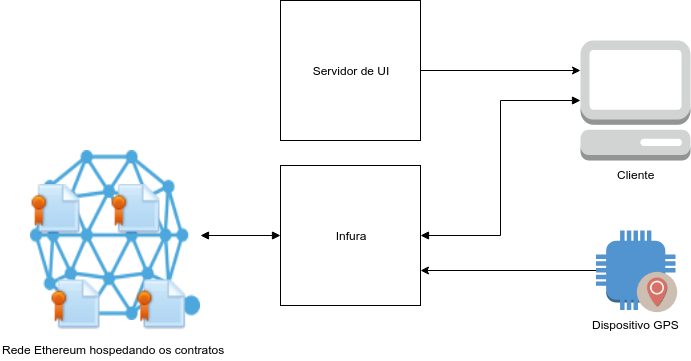
\includegraphics[width=0.7\textwidth]{Cap2/full_ethereum_architecture.png}
\caption{Arquitetura baseada 100\% na rede ethereum.}
\label{full_ethereum_architecture}
\end{figure}

Como pode-se observar na figura \ref{full_ethereum_architecture}, essa arquitetura é composta por 5 componentes:

\begin{itemize}
	\item \textbf{Cliente:} O cliente representa a aplicação web desenvolvida com a framework React (\href{http://www.reactjs.org}{http://www.reactjs.org}) e é responsável por criar um interface gráfica na qual as pessoas possam observar e interagir com os contratos de uma forma amigável.
    \item \textbf{Servidor de UI:} É um servidor de recursos estáticos desenvolvido em Nodejs (\href{http://www.nodejs.org}{http://www.nodejs.org}) com a framework Express (\href{http://www.express.com}{http://www.express.com}). Tal servidor provê o arquivo javascript que contém o código do cliente desenvolvido em React, bem como as imagens da aplicação web.
    \item \textbf{Infura:} Infura (\href{https://infura.io/}{https://infura.io/}) é um serviço web que prove acesso a rede Ethereum por meio de uma API REST. Esse serviço abstrai a complexidade de criar e manter um nó próprio conectado a rede Ethereum.
    \item \textbf{Rede Ethereum:} Representa a rede Ethereum composta por nós espalhados pelo mundo todo.
    \item \textbf{Contratos:} Representa os contratos de seguro automotivo criados e mantidos pelos usuários da aplicação.
    \item \textbf{Dispositivo GPS:} O dispositivo GPS é responsável por enviar constantemente a localização do carro dos participantes do contrato de seguro automotivo para a rede Ethereum. Para manter a privacidade dos usuários, o envio da latitude e longitude é criptografado.
\end{itemize}

Nas seções abaixo, será dado enfoque nos principais componentes do sistema: os contratos, o cliente e o dispositivo GPS.

\subsection{Contratos}

Foram desenvolvidos dois contratos inteligentes, o primeiro deles, SmartCarInsuranceContractFactory, é um contrato responsável por criar e rastrear todos contratos de seguro automotivo. Já o segundo contrato desenvolvido, SmartCarInsuranceContract, representa o próprio contrato de seguro automotivo. O código completo dos contratos está disponível no GitHub (\href{https://github.com/marcoprado17/scife-contracts}{https://github.com/marcoprado17/scife-contracts}).

\begin{figure}[h!]
\centering
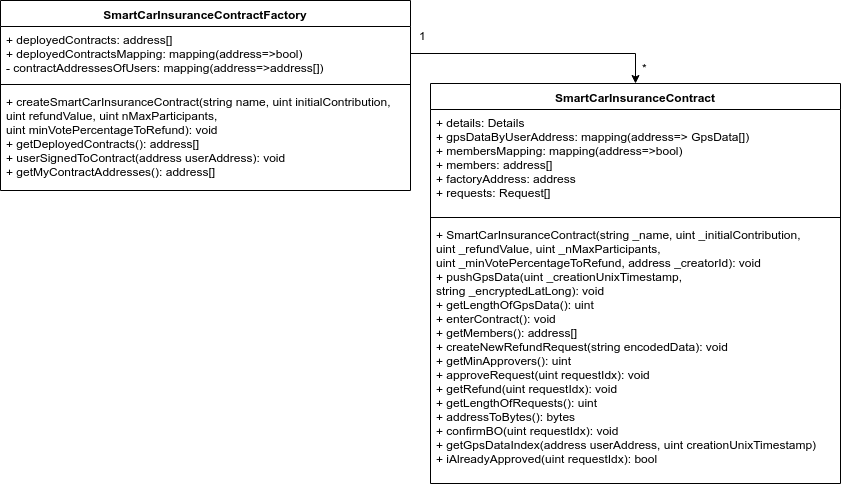
\includegraphics[width=1\textwidth]{Cap2/SmartCarInsuranceContractFactory_and_SmartCarInsuranceContract.png}
\caption{SmartCarInsuranceContractFactory e SmartCarInsuranceContract.}
\label{factory_and_contracts}
\end{figure}

Utilizar um contrato que cria outros contratos é interessante por dois motivos:

\begin{enumerate}
\item Facilita com que os usuários façam o deploy de um novo contrato automotivo no próprio browser. Para tanto, o código do cliente interage com SmartCarInsuranceContractFactory por meio do serviço do Infura para criar um novo contrato;
\item Como todo novo SmartCarInsuranceContract é criado por SmartCarInsuranceContractFactory, o próprio contrato SmartCarInsuranceContractFactory se torna o local ideal para armazenar todos os SmartCarInsuranceContract criados.
\end{enumerate}

Conforme se observa na figura \ref{factory_and_contracts}, um contrato se asemelha muito a uma classe em uma linguagem orientada a objetos: o contrato define um modelo de uma entidade que possui diferentes atributos e métodos. Tal modelo da origem a múltiplas instâncias dessa entidade, sendo que cada instância de contrato criado possui um endereço associado na rede Ethereum.

\subsubsection{SmartCarInsuranceContractFactory}

Segue abaixo o código comentado do contrato SmartCarInsuranceContractFactory:

\begin{code}
\begin{minted}[
frame=lines,
fontsize=\footnotesize,
linenos
]{javascript}
// Utilizando a versão 0.4.17 da linguagem Solidity
pragma solidity ^0.4.17;

contract SmartCarInsuranceContractFactory {
    // Array contendo os endereços ethereum de todos os contratos 
    // SmartCarInsuranceContract que SmartCarInsuranceContractFactory 
    // gerou
    address[] public deployedContracts;
    // Hash table para checagem rápida se certo endereço 
    // ethereum representa um contrato SmartCarInsuranceContract 
    // deployado por SmartCarInsuranceContractFactory
    mapping(address => bool) public deployedContractsMapping;
    // Mapeia os contratos SmartCarInsuranceContract que cada 
    // usuário participa
    mapping(address => address[]) contractAddressesOfUsers;

    // Método que cria uma nova instância de SmartCarInsuranceContract
    function createSmartCarInsuranceContract(
        string name,
        uint initialContribution,
        uint refundValue,
        uint nMaxParticipants,
        uint minVotePercentageToRefund
    ) public {
        // Criando uma nova instância de um contrato 
        // SmartCarInsuranceContract
        address newContractAddress = new SmartCarInsuranceContract(
            name,
            initialContribution,
            refundValue,
            nMaxParticipants,
            minVotePercentageToRefund, 
            msg.sender
        );
        // Armazenando o contrato deployado em deployedContracts
        deployedContracts.push(newContractAddress);
        // Adicionando à hash table deployedContractsMapping o 
        // endereço do novo contrato deployado
        deployedContractsMapping[newContractAddress] = true;
    }

    // Obtenção de deployedContracts
    function getDeployedContracts() public view returns (address[]) {
        return deployedContracts;
    }

    // Adiciona à contractAddressesOfUsers que userAddress agora faz 
    // parte do contrato SmartCarInsuranceContract que chamou essa 
    // função (msg.sender)
    function userSignedToContract(address userAddress) public{
        // Garantindo que quem chamou userSignedToContract seja de 
        // fato um contrato SmartCarInsuranceContract deployado 
        // por SmartCarInsuranceContractFactory
        require(deployedContractsMapping[msg.sender]);
        contractAddressesOfUsers[userAddress].push(msg.sender);
    }

    // Obtendo a array contendo os endereços dos contratos 
    // SmartCarInsuranceContract que o usuário que chamou essa 
    // função participa
    function getMyContractAddresses() public view returns (address[]){
        return contractAddressesOfUsers[msg.sender];
    }
}
\end{minted}
\caption{SmartCarInsuranceContractFactory}
\label{lst:SmartCarInsuranceContractFactory}
\end{code}

\subsubsection{SmartCarInsuranceContract}

Segue abaixo o código comentado de SmartCarInsuranceContract:

\begin{code}
\begin{minted}[
frame=lines,
fontsize=\footnotesize,
linenos
]{javascript}
contract SmartCarInsuranceContract {
    // Definindo a struct Details, tal struct armazena 
    // os principais dados do contrato
    struct Details {
        // Nome do contrato
        string name;
        // Contribuição inicial para participar do contrato
        uint initialContribution;
        // Valor do reembolso em caso de furto e roubo
        uint refundValue;
        // Número máximo de participantes
        uint nMaxParticipants;
        // Percentagem mínima de votos para liberar
        // o reembolso de caso de roubo ou furto
        uint minVotePercentageToRefund;
        // Endereço ethereum do criador desse contrato
        address creatorId;
        // Número de participantes do contrato
        uint nParticipants;
    }

    // Definindo a struct GpsData, tal struct armazena
    // uma amostra dos dados de gps de um usuário do contrato
    struct GpsData {
        // Unix timestamp do bloco ethereum que recebeu 
        // tal GpsData
        uint blockUnixTimestamp;
        // Tempo em que tal amostra foi colhida, esse valor
        // é enviado pelo usuário
        uint creationUnixTimestamp;
        // String encriptada contendo a latitude e longitude 
        // dessa amostra de sinal gps
        string encryptedLatLong;
    }

    // Definindo a struct Request, tal struct representa
    // uma requisição de reembolso criado por um usuário
    // do contrato
    struct Request {
        // String base64 encoded contendo um json com as informações
        // necessárias para a requisição:
        // {
        //     unixTimesptampOfTheft: 1232143213,
        //     latTheft: 1.2231
        //     longTheft: 2.2314
        //     keysOfGpsData = [
        //         [122348763244, "secret"], # [unixTimestamp, key]
        //         [122348763244, "secret"],
        //         ...
        //     ]
        // }
        string encodedData;
        // Endereço ethereum de quem criou a requisição de reembolso
        address creatorAddress;
        // Hash table que mapeia o endereço ethereum de quem aprovou
        // tal requisição de reembolso
        mapping(address => bool) approvers;
        // Número de usuários que aprovaram tal requisição de 
        // reembolso
        uint nApprovers;
        // Bool que indica se tal requisição de reembolso foi
        // aprovada pela polícia
        bool boConfirmed;
        // Unix timestamp do bloco ethereum que recebeu essa
        // nova requisição de reembolso
        uint unixTimestampOfBlock;
        // Bool que indica se o reembolso já foi efetuado ou não
        bool refundMade;
    }

    // Detalhes desse contrato de seguro automotivo
    Details public details;
    // Hash table que armazena os dados de gps de cada
    // membro do contrato
    mapping(address => GpsData[]) public gpsDataByUserAddress;
    // Hash table que armazena o endereço ethereum dos membros
    // do contrato
    mapping(address => bool) public membersMapping;
    // Array com o endereço ethereum de todos os membros do contrato
    address[] public members;
    // Endereço ethereum do contrato SmartCarInsuranceContractFactory
    // que deu origem a este contrato
    address public factoryAddress;
    // Array contento todas as requisições de reembolso feitas
    // nesse contrato
    Request[] public requests;
    
    // Contrutor de SmartCarInsuranceContract. Serve para criar
    // uma nova instância deste contrato
    function SmartCarInsuranceContract(
        string _name,
        uint _initialContribution,
        uint _refundValue,
        uint _nMaxParticipants,
        uint _minVotePercentageToRefund,
        address _creatorId
    ) public {
        // Garantindo alguns requisitos básicos para criação do contrato
        require(_initialContribution > 0);
        require(_refundValue > 0);
        require(_nMaxParticipants > 0);
        require(_minVotePercentageToRefund >= 0 && 
        _minVotePercentageToRefund <= 100);
        // Criando os detalhes desse contrato
        details = Details({
            name: _name,
            initialContribution: _initialContribution,
            refundValue: _refundValue,
            nMaxParticipants: _nMaxParticipants,
            minVotePercentageToRefund: _minVotePercentageToRefund,
            creatorId: _creatorId,
            nParticipants: 0
        });
        // Atualizando o endereço de quem criou a instância desse contrato
        factoryAddress = msg.sender;
    }

    // Método que adiciona um novo GpsData de um membro do contrato
    function pushGpsData(
        uint _creationUnixTimestamp, 
        string _encryptedLatLong) public {
        // Garantindo que quem chamou esse método seja um membro do contrato
        require(membersMapping[msg.sender]);
        uint l = gpsDataByUserAddress[msg.sender].length;
        if(l > 0){
            // Garantindo que unix timestamp fornecido pelo gps
            // seja maior do que o timestamp da última amostra
            // de sinal gps
            require(_creationUnixTimestamp > 
                gpsDataByUserAddress[msg.sender][l-1].creationUnixTimestamp);
        }
        // Criando uma nova instância de GpsData
        GpsData memory newGpsData = GpsData({
            blockUnixTimestamp: block.timestamp,
            creationUnixTimestamp: _creationUnixTimestamp,
            encryptedLatLong: _encryptedLatLong
        });

        // Adicionando a nova instância de GpsData criada para
        // a hash table gpsDataByUserAddress
        gpsDataByUserAddress[msg.sender].push(newGpsData);
    }

    // Método para a obtenção do comprimento da array que armazena
    // os dados de gps de um usuário específico
    function getLengthOfGpsData(address _address) 
    public view returns(uint) {
        return gpsDataByUserAddress[_address].length;
    }

    // Método que um possível membro do contrato chama para participar
    // do contrato de seuro automotivo em questão
    function enterContract() public payable{
        // Garantindo que o possível membro envie, ao chamar essa
        // função, um valor igual a contribuição inicial estabelecida
        // no momento em que esse contrato foi gerado
        require(msg.value == details.initialContribution);
        // Garantindo que quem chamou essa função não seja
        // membro do contrato ainda
        require(!membersMapping[msg.sender]);
        // Garantindo que o contrato em questão ainda não excederá
        // o número máximo de participantes
        require(members.length < details.nMaxParticipants);
        // Incrmentando o número de participantes
        details.nParticipants++;
        // Adicionando o novo membro à membersMapping e members
        membersMapping[msg.sender] = true;
        members.push(msg.sender);
        // Informando a SmartCarInsuranceContractFactory que msg.sender
        // agora é um membro deste contrato
        SmartCarInsuranceContractFactory smartCarInsuranceContractFactory = 
            SmartCarInsuranceContractFactory(factoryAddress);
        smartCarInsuranceContractFactory.userSignedToContract(msg.sender);
    }

    // Obtendo a array com os endereços ethereum dos membros deste contrato
    function getMembers() public view returns (address[]) {
        return members;
    }

    // Método chamado para a criação de uma nova requisição de reembolso
    /*
        encodedData representa a base64 encode do objeto abaixo:
        {
            unixTimesptampOfTheft: 1232143213,
            latTheft: 1.2231
            longTheft: 2.2314
            keysOfGpsData = [
                [122348763244, "secret"], # [unixTimestamp, key]
                [122348763244, "secret"],
                ...
            ]
        }
     */
    function createNewRefundRequest(string encodedData) public {
        // Garantindo que quem chamou esse método (msg.sender)
        // seja um membro do contrato
        require(membersMapping[msg.sender]);
        // Criando uma nova instância da struct Request com
        // os devidos dados
        Request memory newRequest;
        newRequest.encodedData = encodedData;
        newRequest.creatorAddress = msg.sender;
        newRequest.boConfirmed = false;
        newRequest.nApprovers = 0;
        newRequest.unixTimestampOfBlock = block.timestamp;
        newRequest.refundMade = false;
        // Adicionando a instância de request criada à
        // array requests
        requests.push(newRequest);
    }

    // Obtendo o número mínimo de membros que devem aprovar
    // uma requisição de reembolso para ela ser liberada
    function getMinApprovers() public view returns (uint) {
        // Retornando 0 caso details.minVotePercentageToRefund == 0
        if(details.minVotePercentageToRefund == 0) {
            return 0;
        }
        // Retornando ceil de
        // details.minVotePercentageToRefund*details.nParticipants/100
        // caso contrário
        uint multi = details.minVotePercentageToRefund * details.nParticipants;
        bool hasRemainder = true;
        if(multi % 100 == 0){
            hasRemainder = false;
        }
        uint minApprovers = multi / 100;
        if(hasRemainder){
            minApprovers++;
        }
        return minApprovers;
    }

    // Método que um usuário chama para aprovar determinada
    // requisição de reembolso
    function approveRequest(uint requestIdx) public{
        // Garantindo que msg.sender seja um membro do contrato
        require(membersMapping[msg.sender]);
        // Garantindo que msg.sender não tenha aprovado tal
        // requisão antes
        require(!requests[requestIdx].approvers[msg.sender]);
        // Adicionando aos aprovadores da requisição o endereço
        // de msg.sender
        requests[requestIdx].approvers[msg.sender] = true;
        // Aumentando o número de pessoas que aprovaram
        // tal requisição
        requests[requestIdx].nApprovers++;
        // Efetuando o reembolso caso os três requisitos abaxo
        // sejam atendidos
        // a) O número de membros aprovadores do reembolso seja 
        // maior ou igual ao mínimo requerido;
        // b) O contrato possua uma quantia de ethereum maior ou igual
        // ao valor do reembolso;
        // c) O boletim de ocorrência de furto ou roubo já tenha
        // sido confirmado pela polícia.
        uint minApprovers = getMinApprovers();
        if(
            requests[requestIdx].nApprovers >= minApprovers
            && address(this).balance >= details.refundValue
            && requests[requestIdx].boConfirmed
        ){
            requests[requestIdx].creatorAddress.send(details.refundValue);
            requests[requestIdx].refundMade = true;
        }
    }

    // Liberando o reembolso caso todos os requisitos
    // para liberação do reembolso estejam etendidos
    function getRefund(uint requestIdx) public {
        require(requests[requestIdx].creatorAddress == msg.sender);
        require(requests[requestIdx].boConfirmed);
        uint minApprovers = getMinApprovers();
        require(requests[requestIdx].nApprovers >= minApprovers);
        require(address(this).balance >= details.refundValue);
        requests[requestIdx].creatorAddress.transfer(details.refundValue);
        requests[requestIdx].refundMade = true;
    }

    // Obtendo o comprimento da array requests
    function getLengthOfRequests() public view returns(uint) {
        return requests.length;
    }

    // Função que converte um address para bytes
    function addressToBytes(address _addr) public pure returns(bytes) {
        bytes32 value = bytes32(uint256(_addr));
        bytes memory alphabet = "0123456789abcdef";

        bytes memory str = new bytes(51);
        str[0] = "0";
        str[1] = "x";
        for (uint i = 0; i < 20; i++) {
            str[2+i*2] = alphabet[uint(value[i + 12] >> 4)];
            str[3+i*2] = alphabet[uint(value[i + 12] & 0x0f)];
        }
        return str;
    }

    // Função que confirma se o BO de furto ou roubo
    // de uma determinada requisição de reembolso foi feito
    // com sucesso
    function confirmBO(uint requestIdx) public {
        // Garantindo que o BO ainda não tenha sido confirmado
        require(!requests[requestIdx].boConfirmed);
        // Garantindo que msg.sender == 
        // "0x5e924ac15745b75e0d23afd68d1bb1adb8f43689"
        bytes memory validBoSenderAddress = 
        "0x5e924ac15745b75e0d23afd68d1bb1adb8f43689";
        bytes memory senderAddress = addressToBytes(msg.sender);
        bool validSender = true;
        for(uint i = 0; i < validBoSenderAddress.length; i++){
            if(validBoSenderAddress[i] != senderAddress[i]){
                validSender = false;
            }
        }
        require(validSender);
        // Confirmando o BO
        requests[requestIdx].boConfirmed = true;
    }

    // Obtendo o indice do GpsData na array 
    // gpsDataByUserAddress[userAddress] que foi criado
    // o mais proximo possível de creationUnixTimestamp
    function getGpsDataIndex(
        address userAddress, 
        uint creationUnixTimestamp) public view returns(uint){
        if(gpsDataByUserAddress[userAddress].length == 0){
            return 0;
        }
        if(creationUnixTimestamp <= 
        gpsDataByUserAddress[userAddress][0].creationUnixTimestamp){
            return 0;
        }
        if(
            creationUnixTimestamp >= 
            gpsDataByUserAddress[userAddress]
            [gpsDataByUserAddress[userAddress].length-1]
            .creationUnixTimestamp){
            return gpsDataByUserAddress[userAddress].length-1;
        }
        // Efetuando uma busca binária para obtenção do indice
        // de GpsData com creationUnixTimestamp mais próximo
        // do desejado
        uint low = 0;
        uint high = gpsDataByUserAddress[userAddress].length-1;
        while (low <= high) {
            uint mid = (low + high) / 2;
            if(gpsDataByUserAddress[userAddress]
            [mid].creationUnixTimestamp > 
            creationUnixTimestamp){
                high = mid - 1;
            }
            else if (gpsDataByUserAddress[userAddress][mid]
            .creationUnixTimestamp < creationUnixTimestamp){
                low = mid + 1;
            }
            else {
                return mid;
            }
        }
        return low;
    }

    // Método que retorna um bool indicando se msg.sender
    // já aprovou ou não o a requisição de índice requestIdx
    function iAlreadyApproved(uint requestIdx) public view returns (bool) {
        require(membersMapping[msg.sender]);
        return requests[requestIdx].approvers[msg.sender];
    }
}
\end{minted}
\caption{SmartCarInsuranceContract}
\label{lst:SmartCarInsuranceContract}
\end{code}

\subsection{Cliente}

O código do cliente foi desenvolvido com a framework React e encontra-se disponível no GitHub (\href{https://github.com/marcoprado17/scife-ui-service}{https://github.com/marcoprado17/scife-ui-service}). Tal aplicação web contém contém 5 páginas.

\subsubsection{Páginas da aplicação}

\begin{itemize}
\item \textbf{Home Page:} Página principal da aplicação, contém uma explicação básica de como a aplicação e contrato funciona. Um screenshot dessa página pode ser encontrado na figura \ref{home_page}.
\item \textbf{Criação de um novo contrato:} Página que contém um formulário com os dados necessários para a criação de um novo contrato. Um screenshot dessa página pode ser encontrado na figura \ref{new_contract}.
\item \textbf{Participação em um contrato existente:} Página que exibe todos os contratos criados com um botão para o usuário participar do contrato. Um screenshot dessa página pode ser encontrado na figura \ref{participate_existent_contract}.
\item \textbf{Administrar meu contratos:} Página que exibe informações sobre os contratos que o usuário participa. Para cada contrato há 4 abas:
	\begin{itemize}
	\item \textbf{Detalhes:} Informação completa sobre tal contrato. Um screenshot dessa aba pode ser visto na figura \ref{my_contracts_details}
    \item \textbf{Participantes:} Lista o endereço dos participantes do contrato. Um screenshot dessa aba pode ser visto na figura \ref{my_contracts_participants}
    \item \textbf{Requisições:} Lista com as requisições de reembolso feitas por membros do contrato. Nessa aba, o usuário pode aprovar ou não a requisição em questão. Um screenshot dessa aba pode ser visto na figura \ref{my_contracts_requests}
    \item \textbf{Nova Requsição:} Essa aba contém um formulário para que o usuário crie uma nova requisição de reembolso. Um screenshot dessa aba pode ser visto na figura \ref{my_contracts_new_request}
	\end{itemize}
\item \textbf{Confirmação de BO:} Página na qual são exibidos as requisições de reembolso e na qual, apenas a conta Ethereum administrada pela polícia pode aprovar se um boletim de ocorrência condizente com a requisição em questão foi registrado. Um screenshot dessa página pode ser encontrado na figura \ref{confirm_bo}.
\end{itemize}

\begin{figure}[h!]
\centering

\includegraphics[width=0.9\textwidth]{Cap2/home_page.png}
\caption{Home page da aplicação.}
\label{home_page}
\end{figure}

\begin{figure}[h!]
\centering
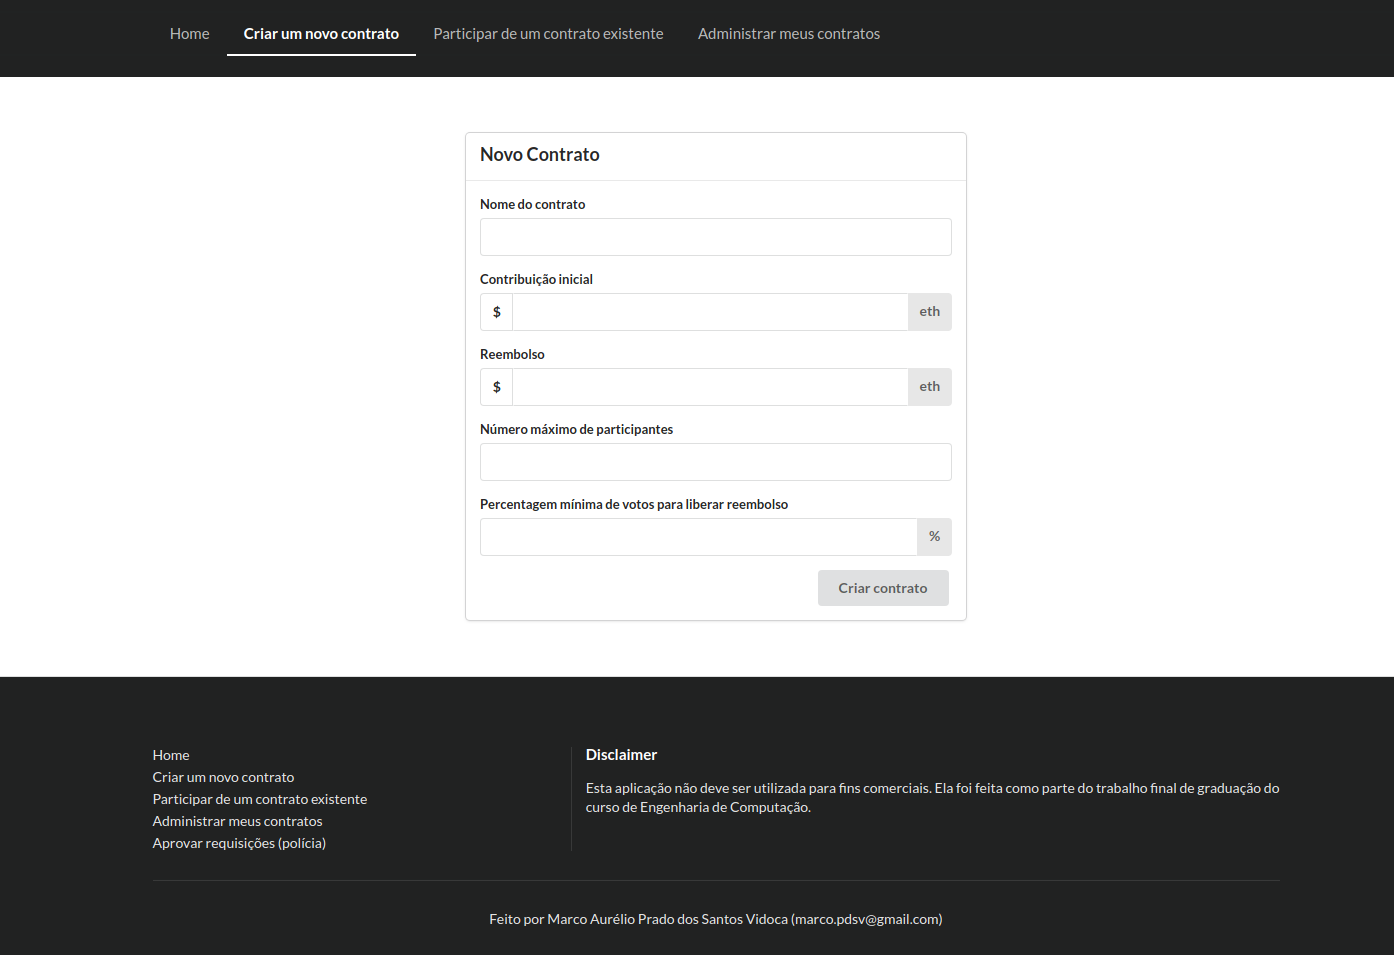
\includegraphics[width=0.9\textwidth]{Cap2/new_contract.png}
\caption{Formulário para a criação de um novo contrato de seguro automotivo.}
\label{new_contract}
\end{figure}

\begin{figure}[h!]
\centering
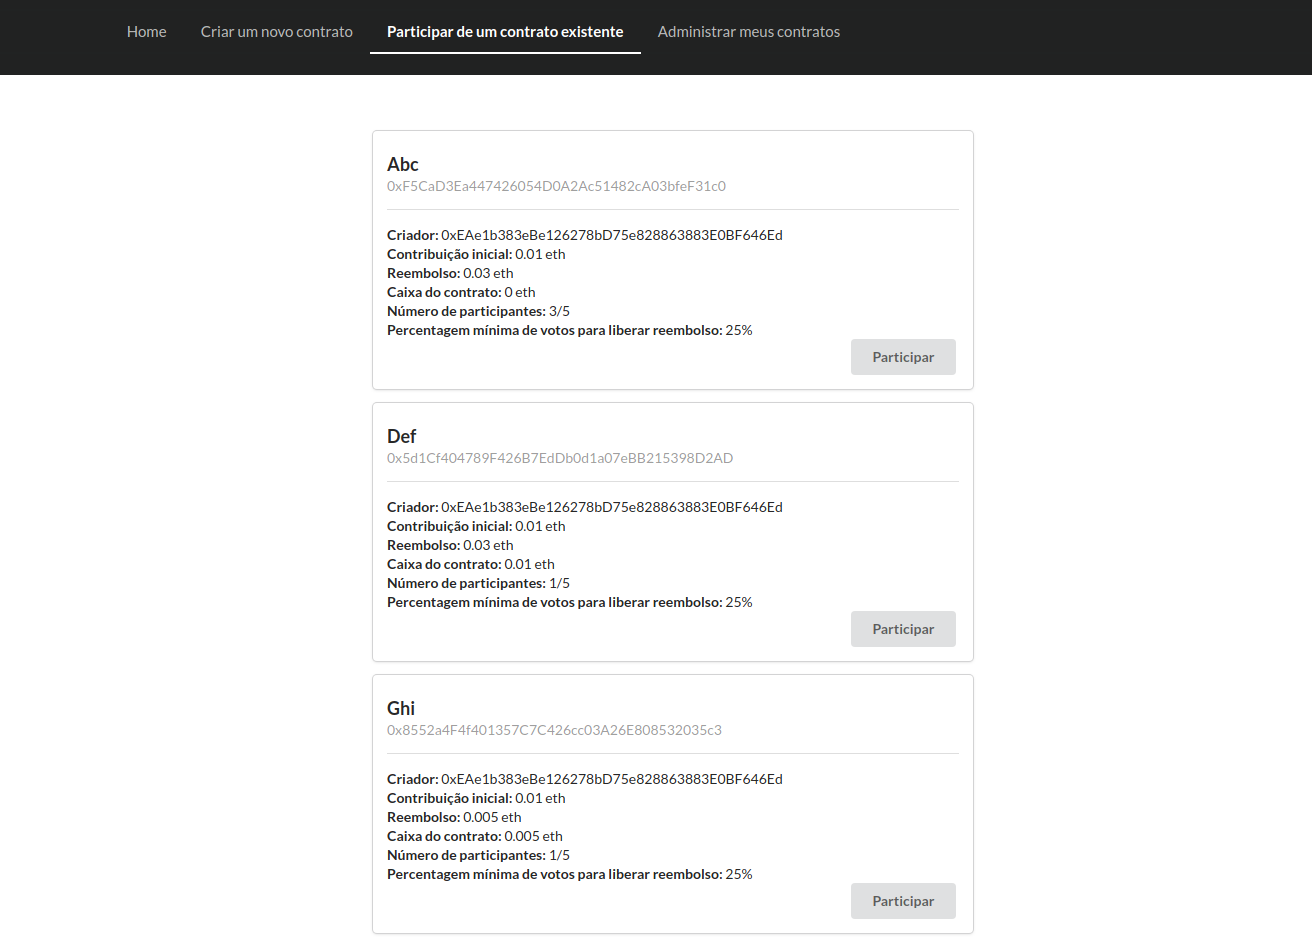
\includegraphics[width=0.9\textwidth]{Cap2/participate_existent_contract.png}
\caption{Lista com os contratos criados e os quais qualquer pessoa pode participar mediante ao pagamento de taxa.}
\label{participate_existent_contract}
\end{figure}

\begin{figure}[h!]
\centering
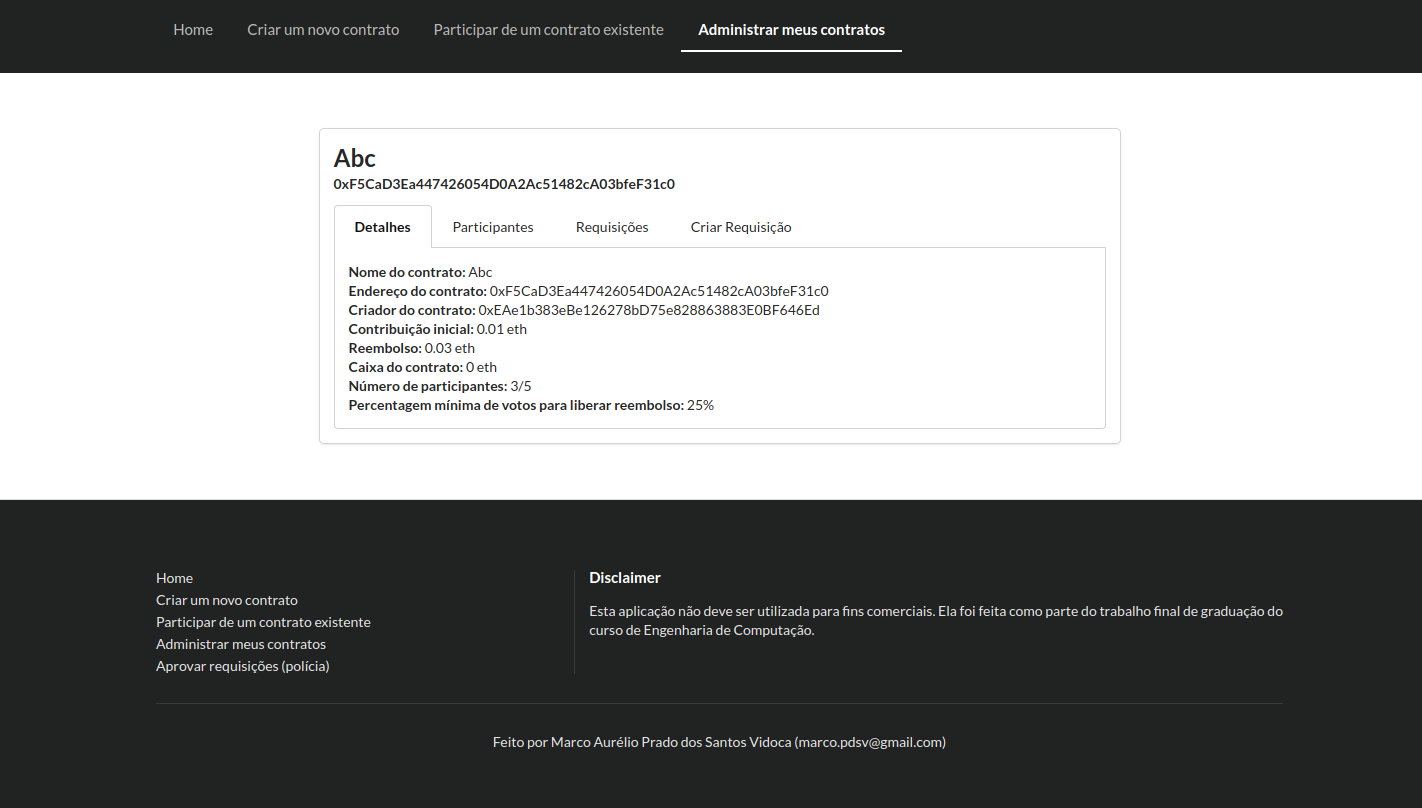
\includegraphics[width=0.9\textwidth]{Cap2/my_contracts_details.png}
\caption{Página contendo os contratos ativos da pessoa que está acessando a aplicação. Nesse caso, se vê a aba de detalhes do contrato.}
\label{my_contracts_details}
\end{figure}

\begin{figure}[h!]
\centering
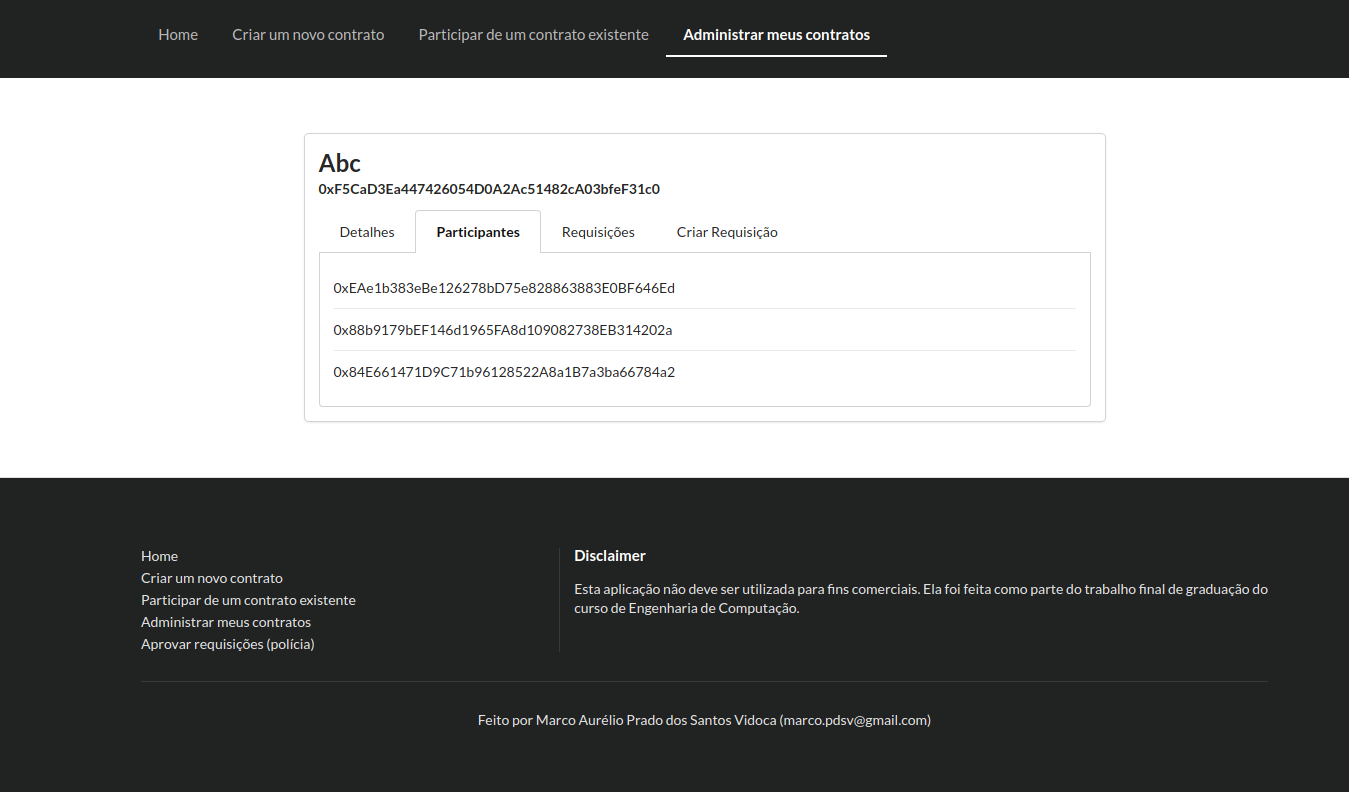
\includegraphics[width=0.9\textwidth]{Cap2/my_contracts_participants.png}
\caption{Página contendo os contratos ativos da pessoa que está acessando a aplicação. Nesse caso, se vê a aba que exibe o endereço da conta Ethereum de quem participa do contrato.}
\label{my_contracts_participants}
\end{figure}

\begin{figure}[h!]
\centering
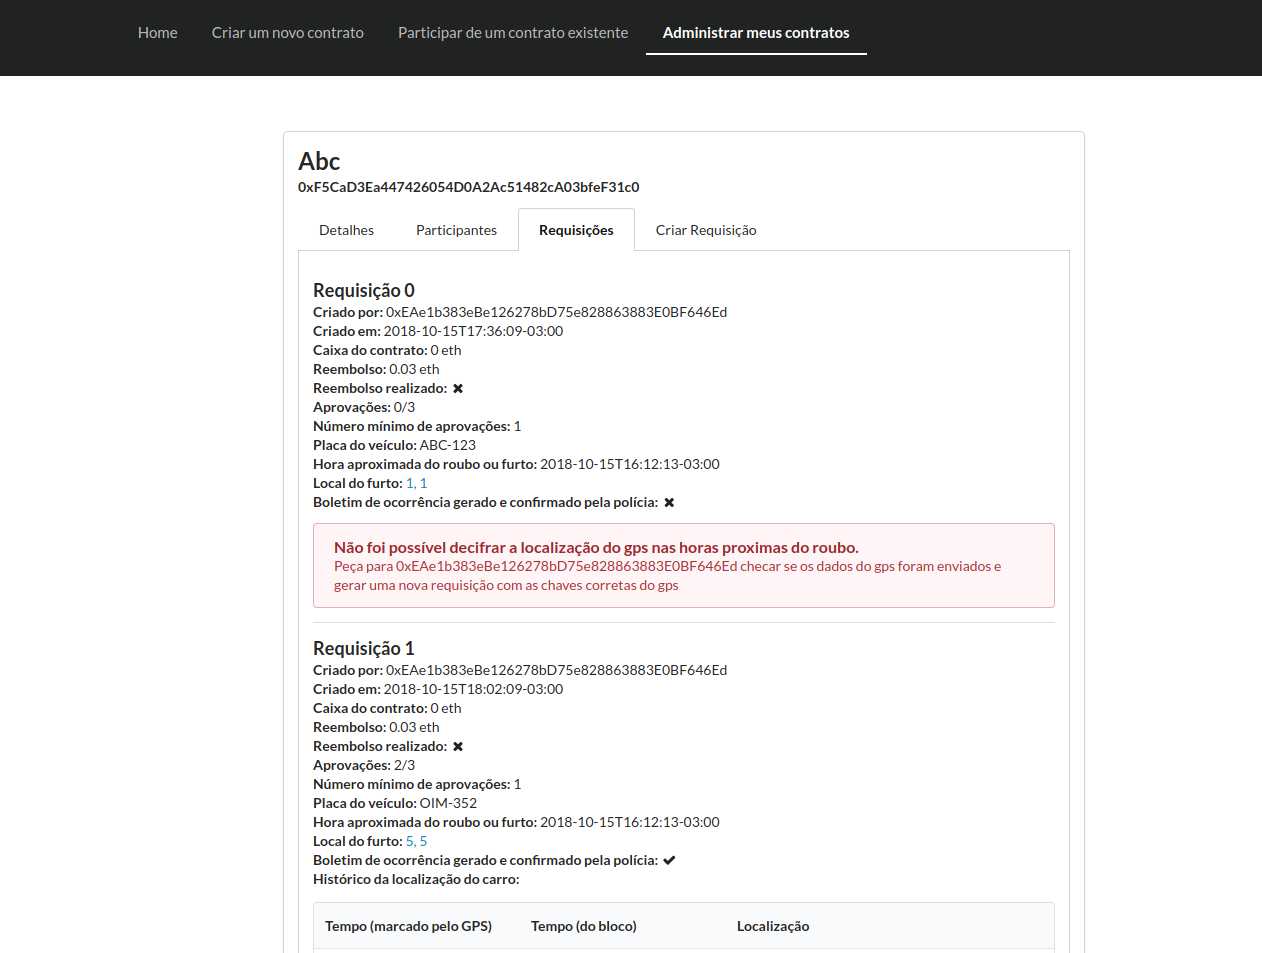
\includegraphics[width=0.9\textwidth]{Cap2/my_contracts_requests.png}
\caption{Página contendo os contratos ativos da pessoa que está acessando a aplicação. Nesse caso, se vê a aba que exibe as requisições de reembolso feitas pelos participantes do contrato.}
\label{my_contracts_requests}
\end{figure}

\begin{figure}[h!]
\centering
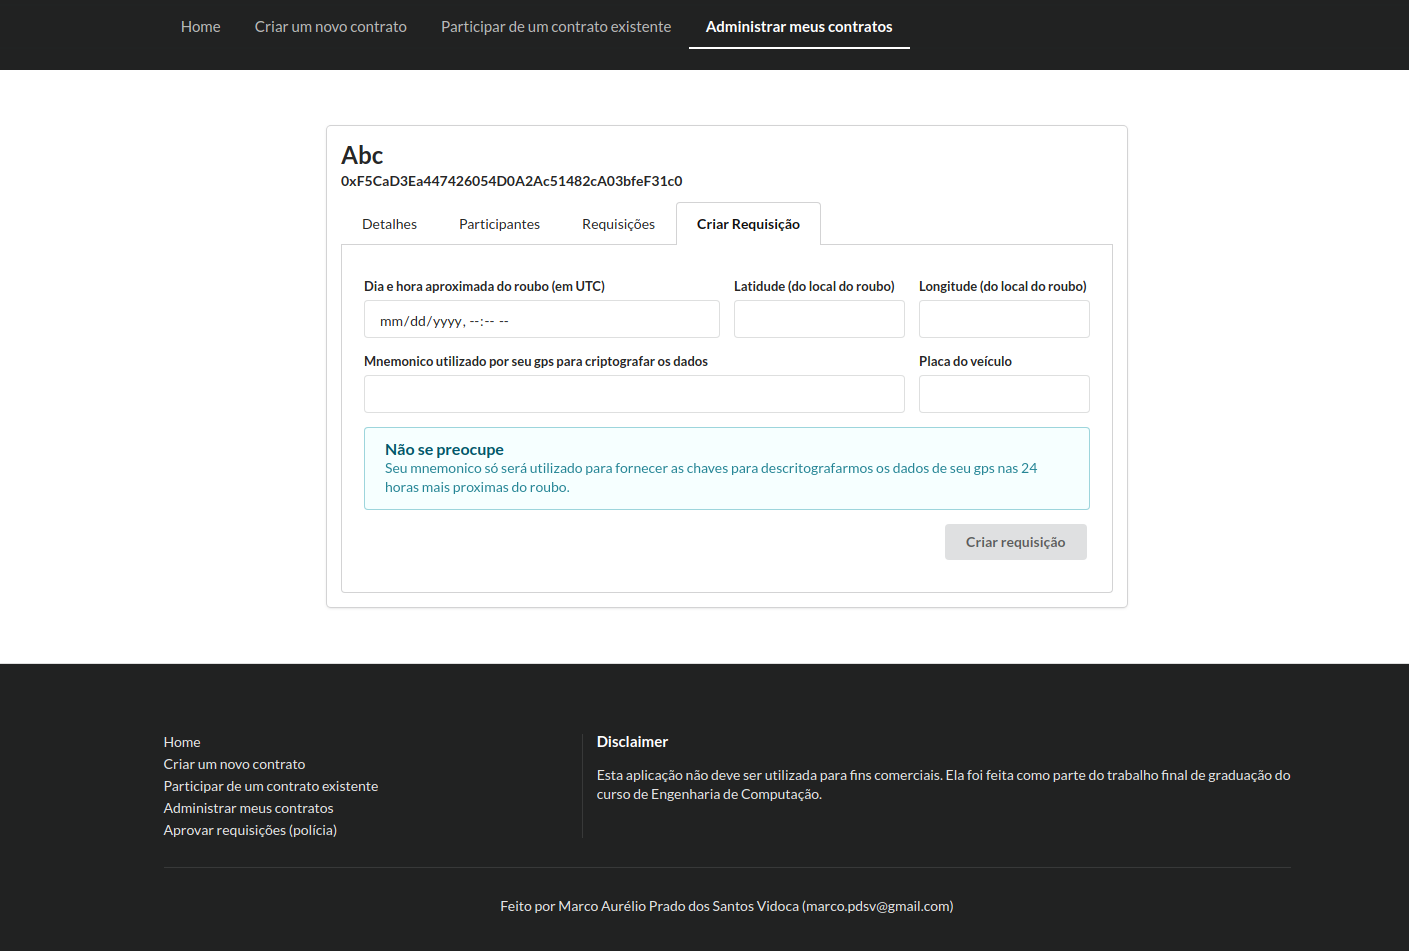
\includegraphics[width=0.9\textwidth]{Cap2/my_contracts_new_request.png}
\caption{Página contendo os contratos ativos da pessoa que está acessando a aplicação. Nesse caso, se vê a aba na qual o participante do contrato pode criar uma nova requisição de reembolso.}
\label{my_contracts_new_request}
\end{figure}

\begin{figure}[h!]
\centering
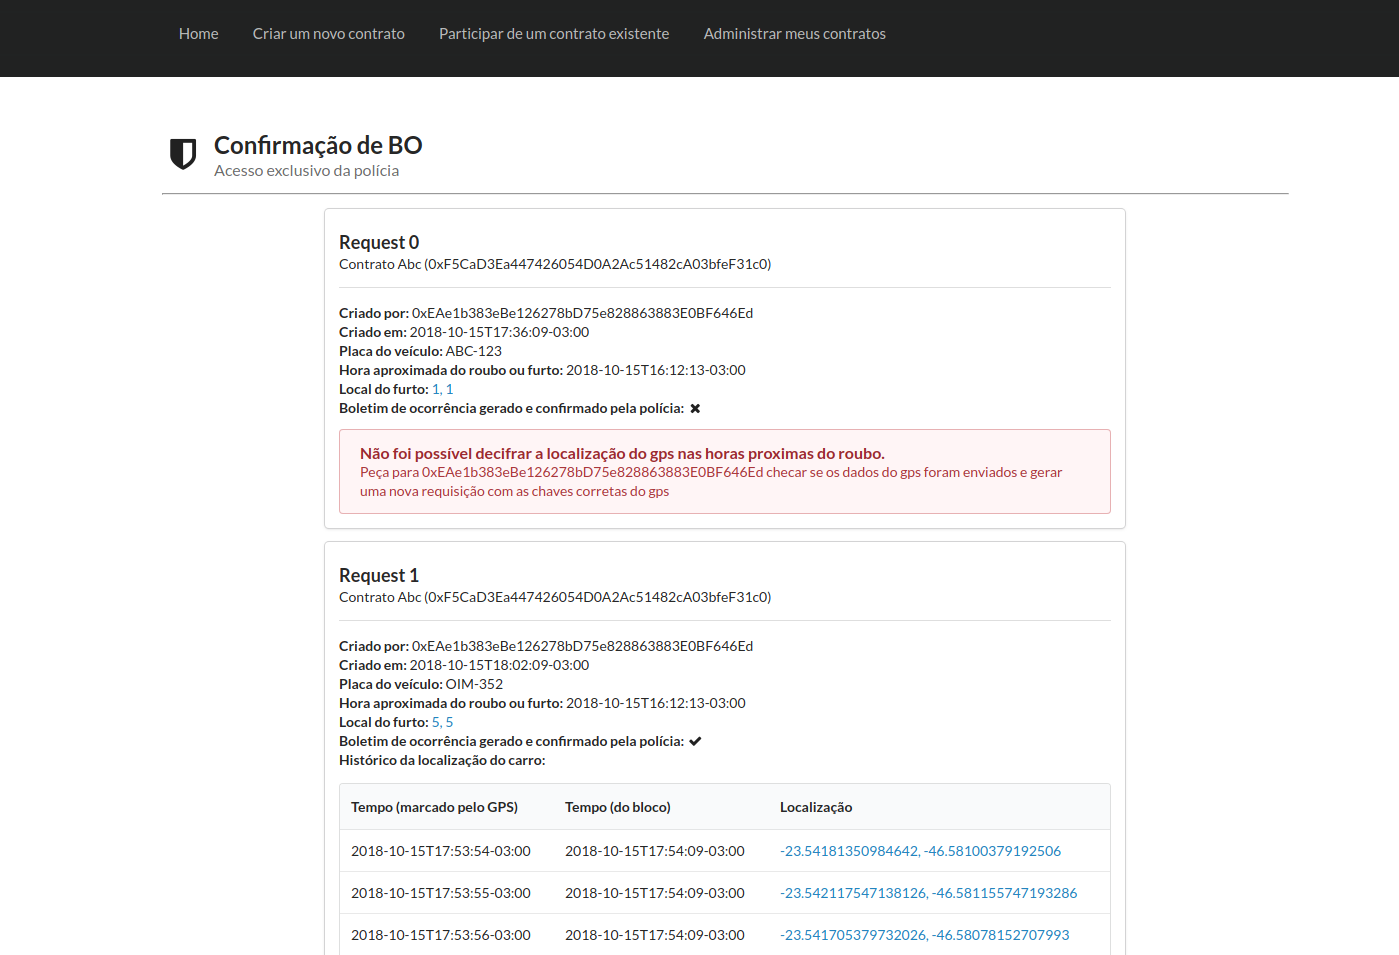
\includegraphics[width=0.9\textwidth]{Cap2/confirm_bo.png}
\caption{Página na qual são exibidos as requisições de reembolso e na qual, apenas a conta Ethereum administrada pela polícia pode aprovar se um boletim de ocorrência condizente com a requisição em questão foi registrado.}
\label{confirm_bo}
\end{figure}

\clearpage
\subsubsection{Comunicação com a Rede Ethereum por meio da lib web3js}

Para a aplicação cliente se comunicar com a rede Ethereum, é utilizada a bliblioteca javascript web3js versão 1.0.0-beta36. Essa biblioteca permite a interação com um nó remoto ou local da rede Ethereum. No código abaixo, pode-se ver como a biblioteca é utilizada na criação de um novo contrato de seguro automotivo:

\begin{code}
\begin{minted}[
frame=lines,
fontsize=\footnotesize,
linenos
]{javascript}
// Importando a lib web3js
import Web3 from 'web3'; 
// Importando o json com as especificações de SmartCarInsuranceContractFactory
import SmartCarInsuranceContractFactory from 
'./build/SmartCarInsuranceContractFactory.json';

// Criando a instância da lib web3 a partir do provedor  do MetaMask
const web3 = new Web3(window.web3.currentProvider);
// Criando uma instância da fábrica de contratos
const smartCarInsuranceContractFactory = new web3.eth.Contract(
    JSON.parse(SmartCarInsuranceContractFactory.interface),
    "0xB7CbfB9d3a64983623f06C410489eA0bCb628B06"
);
// Obtendo as contas cadastradas no MetaMask
const accounts = await web3.eth.getAccounts();

// Chamando o método que cria um novo contrato automotivo, passando
// os parâmetros necessários: nome do contrato, contribuição inicial,
// valor do reembolso, número máximo de participantes e mínima
// percentagem de votos para liberar reembolso
await smartCarInsuranceContractFactory.methods
	.createSmartCarInsuranceContract(
		this.state.contractName,
      	web3.utils.toWei(this.state.initialContribution),
      	web3.utils.toWei(this.state.refundValue),
      	this.state.nMaxParticipants,
      	this.state.minVotePercentageToRefund)
  	.send({
  		from: accounts[0]
	});
\end{minted}
\caption{Biblioteca web3js}
\label{lst:lib_web3js}
\end{code}

Conforme se observa no código acima, o construtor de Web3 recebe window.web3.currentProvider. Para se criar uma instância de um objeto Web3, deve-se passar para o construtor de Web3 um objeto que implemente a interface Provider. Tal objeto é responsável por estabelecer como a lib Web3 irá interagir com o blockchain.

\begin{figure}[h]
\centering
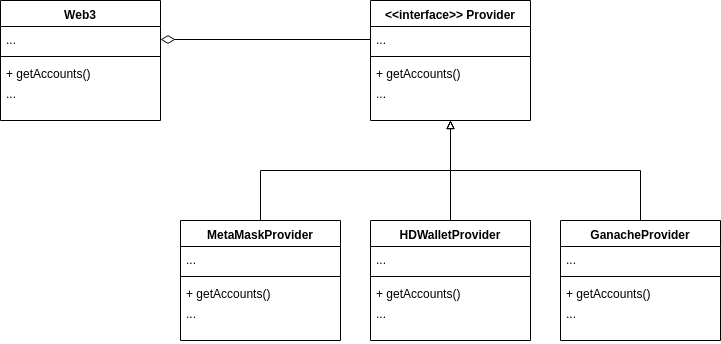
\includegraphics[width=0.7\textwidth]{Cap2/providers.png}
\caption{Strategy pattern com os Providers do Web3.}
\label{providers}
\end{figure}

Na aplicação construída, utilizou-se 3 Providers diferentes:

\begin{itemize}
\item \textbf{MetaMaskProvider:} Metamask é uma extensão do chrome que gerencia as contas dos usuários na rede Ethereum. Ele injeta em toda página web que o usuário visita um Provider com as contas cadastradas pelo usuário e que se comunica com a rede Ethereum utilizando o Infura.
\item \textbf{HDWalletProvider:} Esse provider é utilizado para fazer o deploy de SmartCarInsuranceContractFactory e também na aplicação que simula o gps e envia os dados para o contrato de seuguro automotivo. Esse provider recebe as credenciais da conta Ethereum e a url de accesso do Infura.
\item \textbf{GanacheProvider:} Esse provider é utilizado nos testes dos contratos. O Ganache cria uma rede blockchain Ethereum na máquina local e disponibiliza um provider para se comunicar com rede criada. O Ganache configura tal rede de forma que as transações ocorram rapidamente, criando uma ambiente ideal para testar os contratos antes de fazer o deploy para a rede Ethereum principal.
\end{itemize}

\subsection{Dispositivo GPS}

O dispositivo GPS foi simulado por um código desenvolvido em NodeJs e se encontra disponível no GitHub (\href{https://github.com/marcoprado17/scife-gps-simulator}{https://github.com/marcoprado17/scife-gps-simulator}). O código do simulador foi dividido em dois scripts, o primeiro deles, run.js, é responsável por criar n processos que executam o segundo script, run\_for\_user.js. Esse segundo script, representa o dispositivo GPS de um usuário do sistema e fica constantemente gerando uma latitude e longitude aleatórios a partir de um ponto inicial (figura \ref{gps_location_generator}) para enviar para o contrato após criptografá-los. Seguem abaixo o pseudo código explicando o funcionamento do simulador do dispositivo GPS de um usuário, bem como o código comentado dos principais arquivos:

\begin{enumerate}
\item Obtenção da chave mestre do dispositivo GPS a partir do mnêmonico utilizando o BIP39;
\item Geração inicial da posição do carro, obtendo a latitude a partir de uma distribuição aleatória uniforme entre -23.603244 e -23.504324 e uma longitude a partir de uma distribuição aleatória uniforme entre -46.679381 e -46.561788;
\item Geração de \(\Delta_{lat}\) e \(\Delta_{long}\) a partir de uma distribuição aleatória uniforme entre -0.005 e 0.005;
\item Obtenção das latitudes e longitudes da iteração atual, \(curr_{lat} = curr+{lat} + \Delta_{lat}\) e \(curr_{long} = curr_{long} + \Delta_{long}\);
\item Obtenção Unix Timestamp atual em segundos, \(t_{0}\);
\item Obtenção do índice da chave privada filha a partir da chave privada mestre, \(i = t_{0} - 946684800\). 946684800 representa o Unix Timestamp de 01/01/2000 00:00:00Z. Como a chave mestra pode dar origem a \(2^{32}\) chaves filhas, podemos gerar as chaves privadas que encriptam o dado do sinal GPS até o Unix Timestamp \(t_{1} = 946684800 + 2^{32} = 5241652096\), ou seja, até 02/07/2136 06:28:00Z;
\item Obtenção da chave privada \(k_{priv}\) = i-essima chave filha da chave privada mestre;
\item Encriptação da latitude e longitude do sinal GPS utilizando \(k_{priv}\) e AES256 \cite{aes}.
\item Envio do sinal GPS para o contrato na rede Ethereum;
\item Medição dos dados pertinentes ao envio dessa amostra de sinal GPS para posterior análise.
\end{enumerate}

\begin{figure}[h!]
\centering
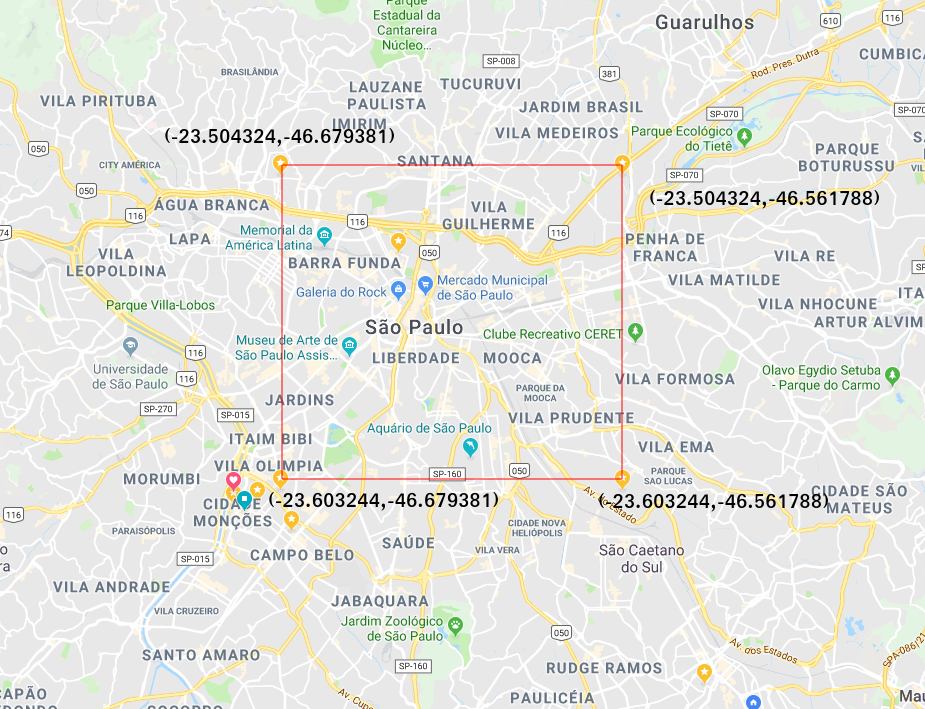
\includegraphics[width=0.9\textwidth]{Cap2/gps_location_generator}
\caption{Posição inicial do sinal GPS do carro de um usuário.}
\label{gps_location_generator}
\end{figure}

\clearpage
\begin{code}
\begin{minted}[
frame=lines,
fontsize=\footnotesize,
linenos
]{javascript}
const spawn = require('child_process').spawn;
// Obtendo o arquivo de configurações
const configs = require('./configs');

[...Array(configs.nUsers).keys()].map(user_idx => {
    // Iniciando um processo que executa o script run_for_user.js
    let command = spawn("node", ["run_for_user.js", user_idx]);
    
    // Imprimindo o stout dos processos filhos no processo mãe
    command.stdout.on('data', function (data) {
        process.stdout.write(data.toString());
    });
    
    // Imprimindo o stderr dos processos filhos no processo mãe
    command.stderr.on('data', function (data) {
        console.log("*** STDERR ***");
        process.stdout.write(data.toString());
    });
    
    // Imprimindo no processo mãe, os processos filhos que finalizaram
    command.on('exit', function (code) {
        console.log('child process exited with code ' + code.toString());
    });
});
\end{minted}
\caption{Script run.js}
\label{lst:run_script}
\end{code}

\clearpage
\begin{code}
\begin{minted}[
frame=lines,
fontsize=\footnotesize,
linenos
]{javascript}
// Obtenção das dependências
const Web3 = require('web3');
const secrets = require('./secrets');
const HDWalletProvider = require('truffle-hdwallet-provider');
const SmartCarInsuranceContract = 
require('./ethereum/build/SmartCarInsuranceContract.json');
const configs = require('./configs');
const Tx = require('ethereumjs-tx');
const bip39 = require("bip39");
const hdkey = require('ethereumjs-wallet/hdkey');
const crypto = require('crypto');
const fs = require('fs');

// Obtenção do indice que representa esse usuário
const user_idx = parseInt(process.argv[2]);

// Obtenção do Provider que será utilizado pela lib web3js para 
// comunicação com o nó Ethereum remoto por meio do Infura
const provider = new HDWalletProvider(
    secrets.mnemonic,
    secrets.infuraUrl,
    user_idx
);

const privKeyBuffer = provider.wallet._privKey;
const accountAddress = provider.address;
const web3 = new Web3(provider);
// Obtenção do contrato
const smartCarInsuranceContract = 
new web3.eth.Contract(
    JSON.parse(SmartCarInsuranceContract.interface), configs.contractAddress);

let nTransactions = 0;

// Obtenção da latitude e longitude inicial
let currentLat = configs.minInitialLat + 
    (configs.maxInitialLat-configs.minInitialLat)*Math.random();
let currentLong = configs.minInitialLong + 
    (configs.maxInitialLong-configs.minInitialLong)*Math.random();

// Obtenção da Hierarchical Deterministic wallet a partir do 
// mnemônico que gerará a seed
const masterSeed = bip39.mnemonicToSeed(secrets.gpsMnemonic);
const gpsHdwallet = hdkey.fromMasterSeed(masterSeed);

// Configurações iniciais do objeto que representa o relatório
let report = {};
report.configs = configs;
report.data = [];

let initialNonce = 0;

// Função que converte uma array de bytes para uma string em hexadecimal 
let decodeHexStringToByteArray = function(hexString) {
    // console.log(hexString);
    var result = [];
    while (hexString.length >= 2) { 
        result.push(parseInt(hexString.substring(0, 2), 16));
        hexString = hexString.substring(2, hexString.length);
    }
    // console.log(result);
    return result;
};

(async function(){
    initialNonce = await web3.eth.getTransactionCount(accountAddress);

    console.log(`initialNonce: ${initialNonce}`);

    // Aguardando certo intervalo de tempo para começar a enviar 
    //os dados do gps
    setTimeout(() => {
    // Enviando os dados do GPS a cada 
    // configs.sendLocationPeriodInMiliseconds milisegundos
    setInterval(async () => {
    try {
        // Incrmentando a transação
        let thisTransaction = nTransactions++;

        // Obtendo o Unix Timestamp atual em segundos
        const currentUnixTimestamp = Math.floor(Date.now()/1000);

        // Obtendo a latitude e longitude dessa iteração
        latLongData = {
            lat: currentLat,
            long: currentLong
        }

        // Setando a latitude e longitude da próxima iteração
        currentLat += (Math.random() > 0.5 ? 1 : -1)*
        Math.random()*configs.maxCoordinateDeltaBetweenCalls;
        currentLong += (Math.random() > 0.5 ? 1 : -1)*
        Math.random()*configs.maxCoordinateDeltaBetweenCalls;

        let thisLat = currentLat;
        let thisLong = currentLong;

        // Obtendo o indice da chave privada filha que será 
        // utilizada para encriptar o sinal GPS dessa iteração
        const i = currentUnixTimestamp-946684800;
        const key = gpsHdwallet
        .deriveChild(i).getWallet().getPrivateKey();

        // Encriptando os dados do GPS com AES256
        const cipher = crypto.createCipher("aes256", key)
        let encryptedGpsData = cipher.update(
            JSON.stringify(latLongData),'utf8','hex'
        );
        encryptedGpsData += cipher.final('hex');

        // Obtendo os dados da transação Ethereum que será 
        // utilizado para chamar a função do nosso contrato 
        // que recebe o sinal GPS
        const data = smartCarInsuranceContract.methods
            .pushGpsData(currentUnixTimestamp, encryptedGpsData)
            .encodeABI();
        let dataAsByteArray = decodeHexStringToByteArray(
            data.substr(2)
        );
        let nNonZeroBytes = 0;
        let nZeroBytes = 0;
        dataAsByteArray.map((byte) => {
            if(byte == 0){
                nZeroBytes++;
            }
            else{
                nNonZeroBytes++;
            }
        });
        // console.log(`nZeroBytes: ${nZeroBytes}`);
        // console.log(`nNonZeroBytes: ${nNonZeroBytes}`);

        const nonce = initialNonce + thisTransaction;

        // Setando os dados da transação
        const txData = {
            nonce: web3.utils.toHex(nonce),
            gasLimit: web3.utils.toHex(1000000),
            gasPrice: web3.utils.toHex(1e9), // 1 Gwei
            to: configs.contractAddress,
            from: accountAddress,
            data: data
        };

        // console.log(txData);

        // Assinando a transação com a chave privada
        const transaction = new Tx(txData);
        transaction.sign(privKeyBuffer);
        const serializedTx = transaction.serialize().toString('hex');
        const sendTxUnixTimestamp = Math.floor(Date.now()/1000);
        web3.eth.sendSignedTransaction('0x' + serializedTx)
            .once('transactionHash', function(hash) {
                console.log(hash);
            })
            .on('error', function(err) {
                // Adicionando os dados dessa transação mal 
                // sucedida ao relatório

                let msg = "";
                msg += `Sending transaction ${thisTransaction}/${nonce} 
                for user ${user_idx} (${accountAddress}) at 
                ${currentUnixTimestamp}\n`;
                msg += `ERROR: ${err.message}`;
                console.log(msg);

                const finishTxUnixTimestamp = Math.floor(Date.now()/1000);
                report.data.push({
                    idx: thisTransaction,
                    status: "ERROR",
                    message: err.message,
                    creationUnixTimestamp: currentUnixTimestamp,
                    lat: thisLat,
                    long: thisLong,
                    encryptedGpsData: encryptedGpsData,
                    sendTxUnixTimestamp: sendTxUnixTimestamp,
                    finishTxUnixTimestamp: finishTxUnixTimestamp,
                    latency: (finishTxUnixTimestamp-sendTxUnixTimestamp),
                    txData: txData,
                    nNonZeroBytes: nNonZeroBytes,
                    nZeroBytes: nZeroBytes
                });
            })
            .then(function(result) {
                // Adicionando os dados dessa transação bem 
                // sucedida ao relatório

                let msg = "";
                msg += `Sending transaction ${thisTransaction}/${nonce} 
                for user ${user_idx} (${accountAddress}) at 
                ${currentUnixTimestamp}\n`;
                msg += `SUCCESS:\n`;
                msg += `${JSON.stringify(result, null, 4)}`;
                console.log(msg);

                const finishTxUnixTimestamp = Math.floor(Date.now()/1000);
                report.data.push({
                    idx: thisTransaction,
                    status: "OK",
                    creationUnixTimestamp: currentUnixTimestamp,
                    lat: thisLat,
                    long: thisLong,
                    encryptedGpsData: encryptedGpsData,
                    sendTxUnixTimestamp: sendTxUnixTimestamp,
                    finishTxUnixTimestamp: finishTxUnixTimestamp,
                    latency: (finishTxUnixTimestamp-sendTxUnixTimestamp),
                    txData: txData,
                    result: result,
                    nNonZeroBytes: nNonZeroBytes,
                    nZeroBytes: nZeroBytes
                });
            });
    }
    catch(err){
        console.error(err);
    }
    }, configs.sendLocationPeriodInMiliseconds);
    }, Math.random() * configs.sendLocationPeriodInMiliseconds);
}());

// Enviando para um arquivo .json os dados do relatório 
// a cada 15 segundos
setInterval(function(){
    const currentUnixTimestamp = Math.floor(Date.now()/1000);
    console.log(`Saving report (${currentUnixTimestamp}.json)...`);
    let stringfiedReport = JSON.stringify(report, null, '\t');
    console.log("report.data.length", report.data.length);
    console.log("Report stringfied");
    // console.log(stringfiedReport);
    fs.writeFileSync(
        `./temp_reports/${currentUnixTimestamp}.json`, 
        stringfiedReport, 'utf-8'
    );
    console.log(`Report ${currentUnixTimestamp}.json saved`);
}, 15000);
\end{minted}
\caption{Script run\_for\_user.js}
\label{lst:run_for_user_script}
\end{code}

\section{Construção do seguro automotivo utilizando a arquitetura híbrida}

\begin{figure}[h]
\centering
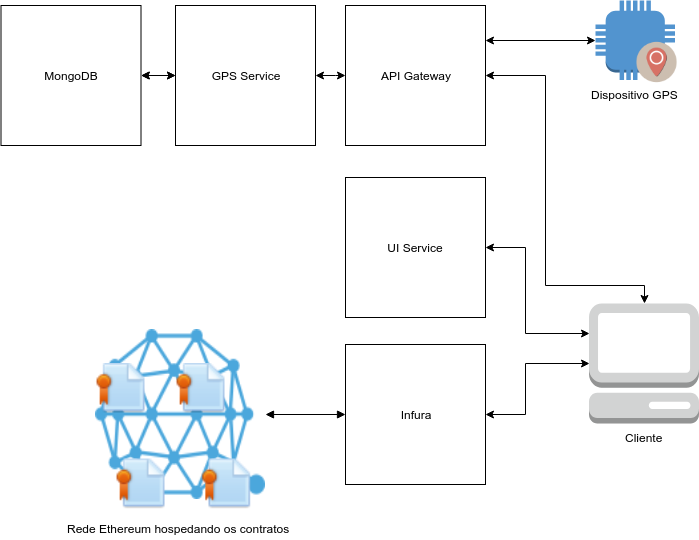
\includegraphics[width=0.9\textwidth]{Cap2/architecture_hybrid.png}
\caption{Arquitetura híbrida.}
\label{architecture_hybrid}
\end{figure}

Como pode-se observar na figura \ref{architecture_hybrid}, essa arquitetura é composta por 8 componentes:

\begin{itemize}
	\item \textbf{Cliente:} O cliente representa a aplicação web que os usuários do seguro utilizam para interagirem com os contratos e com o GPS Service. Devido a semelhança que tal aplicação possue com o cliente da arquitetura 100\% Ethereum e devido ao fato de aplicação cliente não ser necessária para análise proposta, tal componente não foi desenvolvido;
    \item \textbf{Servidor de UI:} É o servidor de recursos estáticos que provê o arquivo javascript que contém o código do cliente, bem como as imagens da aplicação web;
    \item \textbf{Infura:} Infura (\href{https://infura.io/}{https://infura.io/}) é um serviço web que prove acesso a rede Ethereum por meio de uma API REST. Esse serviço abstrai a complexidade de criar e manter um nó próprio conectado a rede Ethereum;
    \item \textbf{Rede Ethereum:} Representa a rede Ethereum composta por nós espalhados pelo mundo todo;
    \item \textbf{Contratos:} Representa os contratos de seguro automotivo criados e mantidos pelos usuários da aplicação. Os contratos dessa arquitetura são semelhantes aos contratos da arquitetura 100\% Ethereum, a diferença é que não possuiriam a função que recebe os dados do GPS e nem a estrutura de dados que armazena os dados do GPS. Devido a tal semelhança, os contratos para a arquitetura híbrida não foram desenvolvidos;
    \item \textbf{Dispositivo GPS:} O dispositivo GPS é responsável por enviar constantemente a localização do carro dos participantes do contrato de seguro automotivo para o GPS Service. Para manter a privacidade dos usuários, o envio da latitude e longitude é criptografado. O código que simula o dispositivo GPS está disponível no GitHub (\href{https://github.com/marcoprado17/scih-gps-simulator}{https://github.com/marcoprado17/scih-gps-simulator}). A única diferença em relação ao simulador de GPS da arquitetura 100\% Ethereum é o envio dos dados do GPS para o API Gateway com uma requisição http do tipo POST, como pode ser visto no código \ref{scih_gps_sim_diff};
    \item \textbf{API Gateway:} Serviço responsável por verificar a autenticidade dos dados enviados pelos dispositivo GPS. Esse serviço também é responsável por direcionar os dados do GPS para o GPS Service. O Código completo desse serviço está disponível no GitHub (\href{https://github.com/marcoprado17/scih-api-gateway}{https://github.com/marcoprado17/scih-api-gateway});
    \item \textbf{GPS Service:} Serviço responsável por interagir com o banco de dados MongoDB para armazenamento dos dados do GPS. O Código completo desse serviço está disponível no GitHub (\href{https://github.com/marcoprado17/scih-gps-service}{https://github.com/marcoprado17/scih-gps-service});
    \item \textbf{MongoDB:} Banco de dados MongoDB versão 3.6.2.
\end{itemize}

\clearpage
\begin{code}
\begin{minted}[
frame=lines,
fontsize=\footnotesize,
linenos
]{javascript}
axios.post(`http://35.239.45.68:81/api/accounts/${accountAddress}/
	contracts/${configs.contractAddress}/gps-data`, {
  data,
  v,
  r,
  s,
  from: accountAddress
})
\end{minted}
\caption{Envio dos dados do GPS para o API Gateway com o uso da biblioteca axios do nodejs}
\label{lst:scih_gps_sim_diff}
\end{code}

	Nas próximas seções será detalhado a implementação dos principais componentes do sistema: API Gateway e GPS Service.

\subsection{Implementação comentada do API Gateway}

\begin{code}
\begin{minted}[
frame=lines,
fontsize=\footnotesize,
linenos
]{javascript}
// Obtenção das dependências
var express = require('express');
var router = express.Router();
const httpProxy = require('express-http-proxy');
const { body, param, validationResult } = require('express-validator/check');
var nconf = require('nconf');
const ethereumjs = require('ethereumjs-util');
const wrapAsync = require('./wrap-assync');
const assert = require('assert');

// Returning 200 on / to serve as health check to ingress
// https://cloud.google.com/kubernetes-engine/docs/tutorials/http-balancer#remarks
router.get('/', function(req, res, next) {
  res.sendStatus(200)
});

/* GET home page. */
router.get('/api', function(req, res, next) {
  res.send("Home page da api!!!");
});

/* gps-service rules */
const gpsServiceProxy = httpProxy(nconf.get("gpsServiceHost"));

router.post('/api/accounts/:accountId/contracts/:contractId/gps-data', [
  // Validando o corpo do request
  body("data.encryptedGpsData").isString(),
  body("data.creationUnixTimestamp").isNumeric(),
  body("from").isString(),
  body("v").isNumeric(),
  body("r.type").equals("Buffer"),
  body("r.data").isArray(),
  body("r.data.*").isNumeric(),
  body("s.type").equals("Buffer"),
  body("s.data").isArray(),
  body("s.data.*").isNumeric(),
  param("accountId").isString(),
  param("contractId").isString()
], wrapAsync(async (req, res, next) => {
    // Se ocorreu algum erro de validação, será retornado o código http 400
    const errors = validationResult(req);
    if (!errors.isEmpty()) {
      return res.status(400).json({ errors: errors.array() });
    }

    // Validando a assinatura ECDSA
    let dataHash = await ethereumjs.sha3(JSON.stringify(req.body.data));
    
    let r = new Buffer(req.body.r.data);
    let s = new Buffer(req.body.s.data);

    try {
      const validSign = ethereumjs.isValidSignature(req.body.v, r, s);
      const pubKey  = ethereumjs.ecrecover(
        ethereumjs.toBuffer(dataHash), req.body.v, r, s);
      const addrBuf = ethereumjs.pubToAddress(pubKey);
      const addr    = ethereumjs.bufferToHex(addrBuf);
      assert(validSign);
      assert.equal(req.body.from, addr)
    }
    catch(err) {
      // Caso a assinatura seja inválida, será retornado o código http 400
      return res.status(400).json({ error: err.message });
    }
    
    // Enviando o dado para GPS Service
    gpsServiceProxy(req, res, next);
}));

// Rota utilizada para obtenção dos dados do GPS
router.get('/api/accounts/:accountId/contracts/:contractId/gps-data', 
(req, res, next) => {
  gpsServiceProxy(req, res, next);
});

module.exports = router;
\end{minted}
\caption{Principais endpoints do API Gateway}
\label{lst:api_gateway}
\end{code}

\subsection{Implementação comentada do GPS Service}

\begin{code}
\begin{minted}[
frame=lines,
fontsize=\footnotesize,
linenos
]{javascript}
const mongoose = require('mongoose');
const timestamps = require('mongoose-timestamp');

const GpsDataSchema = new mongoose.Schema({
    data: {
        // Latitude e longitude encriptada
        encryptedGpsData: { 
            type: String,
            required: true,
        },
        // Unix timestamp de quando essa amostra
        // de sinal GPS foi obtida
        creationUnixTimestamp: {   
            type: Number,
            required: true,
        }
    },
    // Endereço de quem enviou tal dado
    from: {
        type: String,
        require: true
    },
    // Reconver id
    v: {
        type: Number,
        required: true
    },
    // Parâmetro r da assinatura ECDSA
    r: {
        type: Buffer,
        required: true
    },
    // Parâmetro s da assinatura ECDSA
    s: {
        type: Buffer,
        required: true
    },
    // Endereço ethreum da conta que envou tal sinal
    accountId: {
        type: String,
        required: true,
    },
    // Endereço Ethereum do contrato
    contractId: {
        type: String,
        required: true,
    },
}, { collection: 'gpsData' })

GpsDataSchema.plugin(timestamps)

module.exports = exports = mongoose.model('GpsData', GpsDataSchema)
\end{minted}
\caption{Esquema que modela como as informações de uma amostra do sinal GPS será armazenada no banco de dados.}
\label{lst:gps_data_schema}
\end{code}

\begin{code}
\begin{minted}[
frame=lines,
fontsize=\footnotesize,
linenos
]{javascript}
const router = new (require('restify-router')).Router();
const GpsDataSchema = require('./model');

// Endpoint para obtenção dos dados do GPS
router.get('/', function (req, res, next) {
	// default limit to 10 docs
	let limit = parseInt(req.query.limit, 10) || 10; 
	// default skip to 0 docs
	let skip  = parseInt(req.query.skip, 10) || 0; 
	let query = req.params || {};

	// remove skip and limit from data to avoid false querying
	delete query.skip
	delete query.limit

	// Obtendo um determinado dado do GPS
	GpsDataSchema
		.find(query)
		.skip(skip)
		.limit(limit)
		.then(allGpsData => {
			res.send(200, allGpsData)
			next()
		})
		.catch(err => {
			res.send(500, err)
		})
});

// Enviando uma amostra do sinal GPS para o banco de dados
router.post('/', function (req, res, next) {
	// console.log(req.params);
	// Adicionando accountId e contractId ao dado que será 
	// armazenado no banco de dados
	let data = Object.assign({}, 
		{ 	
			accountId: req.params.accountId, 
			contractId: req.params.contractId 
		}, req.body) || {}
	// console.log(data);

	// Enviando para o banco de dados o dado
	GpsDataSchema
		.create(data)
		.then(gpsData => {
			res.send(200)
			next()
		})
		.catch(err => {
			res.send(500, err)
		})
});

module.exports = router;
\end{minted}
\caption{Principais endpoints de GPS Service.}
\label{lst:gps_service_endpoint}
\end{code}








